\documentclass{beamer}

\mode<presentation> {
\usetheme{Madrid}
}

\beamertemplatenavigationsymbolsempty

\usepackage{pacman} % Allows you to be the best presentator ever :D

\usepackage{graphicx} % Allows including images
\usepackage{booktabs} % Allows the use of \toprule, \midrule and \bottomrule in tables
\usepackage[utf8]{inputenc}
\usepackage{float}
\usepackage{subcaption}
\usepackage{mathtools}
\usepackage{xcolor}
\usepackage{bm}

%-----------------------------------------------------------------------------
% Packages project-specified
%-----------------------------------------------------------------------------
\DeclareMathOperator{\Tr}{Tr}

%-----------------------------------------------------------------------------

%-----------------------------------------------------------------------------
%	TITLE PAGE
%-----------------------------------------------------------------------------

\title[ML - 2019/20 - Lorenzo Palloni]{Adversarially Constrained Autoencoder Interpolation using Wasserstein Autoencoder}
\subtitle{Machine Learning}
\author{Lorenzo Palloni}
\institute[]{
    University of Florence\\
    \medskip
    \textit{lorenzo.palloni@stud.unifi.it }
}
\date{\today}

\begin{document}

\begin{frame}
\titlepage % Print the title page as the first slide
\end{frame}

%-----------------------------------------------------------------------------
%	PRESENTATION SLIDES
%-----------------------------------------------------------------------------
%   TABLE OF CONTENTS
%-----------------------------------------------------------------------------
%\begin{frame}
%\tableofcontents
%\end{frame}
%-----------------------------------------------------------------------------
%-----------------------------------------------------------------------------
%-----------------------------------------------------------------------------
\begin{frame}
\frametitle{Introduction}
\begin{itemize}
  \item \textbf{Unsupervised Learning} context
  \medskip
  \item We aim to obtain "high-quality" \textbf{interpolations}
  \medskip
  \item An interpolation example:
\end{itemize}
\ \ \ \ \ \ $\overbrace{\ \ \ \ \ \ \ \ \ \ \ \ \ \ \ \ \ \ \ \ \ \ \ \ \ \ \ \ \ \ \ \ \ \ \ \ \ \ \ \ \ \ \ \ \ \ \ \ \ \ \ \ \ \ \ \ \ \ \ \ \ \ \ \ \ \ \ \ \ \ \ \ \ \ \ \ \ \ \ \ \ \ }^{\text{\textit{interpolated points}}}$
\vspace*{-\baselineskip}
\medskip
\begin{center}
  
\includegraphics[width=1.0\textwidth,keepaspectratio]{./figures/perfect_interpolations}
\end{center}
\vspace*{-\baselineskip}
\begin{noindent}
  \rlap{\ \ $\nwarrow$} \hfill \llap{$\nearrow$\ \ }
\end{noindent}

\begin{noindent}
  \rlap{\textit{an endpoint}} \hfill \llap{\textit{another endpoint}}
\end{noindent}
\medskip
\begin{itemize}
  \item An "high-quality" interpolation point have two characteristics:
  \medskip
  \begin{itemize}
    \item is indistinguishable from real data
    \medskip
    \item represent a semantically smooth morphing between the endpoints
  \end{itemize}
\end{itemize}
\end{frame}
%-----------------------------------------------------------------------------
\begin{frame}
\frametitle{Motivation and Techniques}
\begin{itemize}
  \item Uncover underlying structure of dataset
  \item Better representations $\rightarrow$ better results in other tasks
\end{itemize}
\bigskip
\begin{itemize}
  \item Implemented techniques (using pytorch \cite{pytorch}):
  \begin{itemize}
    \item Adversarially Constrained Autoencoder Interpolation (ACAI) \cite{acai}
    \medskip
    \item Wasserstein Autoencoder (WAE) \cite{wae}
    \medskip
    \item Wasserstein-Wassertein Autoencoder (WWAE) \cite{wwae}
  \end{itemize}
\end{itemize}
\end{frame}
%-----------------------------------------------------------------------------
%\begin{frame}
%\frametitle{Techniques implemented (using pytorch)}
%\begin{itemize}
%  \item ACAI (Adversarially Constrained Autoencoder Interpolation)
%  \medskip
%  \item WAE (Wasserstein Autoencoder)
%  \medskip
%  \item WWAE (Wasserstein-Wassertein Autoencoder)
%\end{itemize}
%\end{frame}
%-----------------------------------------------------------------------------
\begin{frame}
\frametitle{ACAI}
\begin{itemize}
  \item Graphical representation of ACAI structure:
\end{itemize}
\begin{center}
  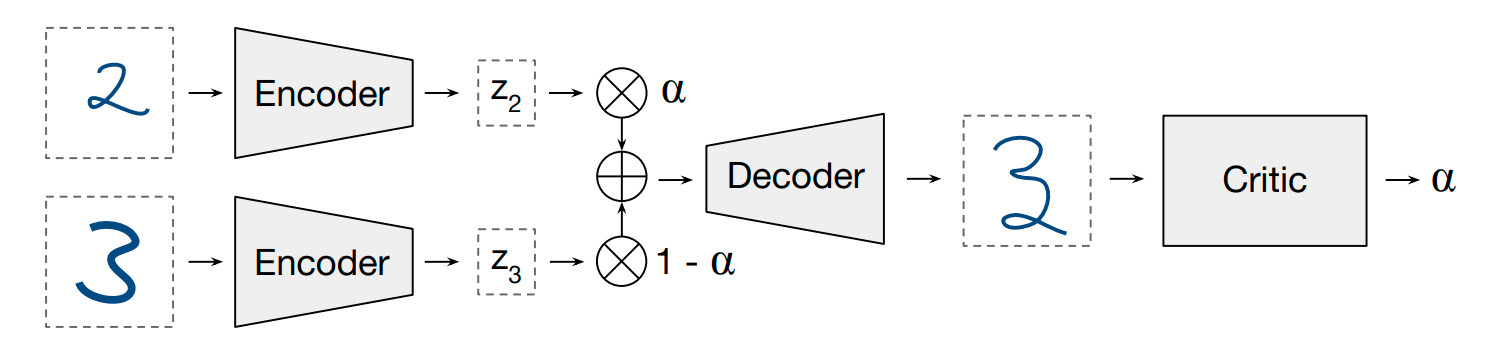
\includegraphics[width=\textwidth,keepaspectratio]{./figures/acai_structure}
\end{center}
\begin{itemize}
  \item Loss functions (discriminator and autoencoder respectively):
\end{itemize}
\begin{align}
  \mathcal{L}_{d}&:=\left\|d_{\omega}\left(\hat{x}_{\alpha}\right)-\alpha\right\|^{2}+\left\|d_{\omega}\left(\gamma x+(1-\gamma) g_{\phi}\left(f_{\theta}(x)\right) \|^{2}\right.\right. \\
  \mathcal{L}_{f, g}&:=\left\|x-g_{\phi}\left(f_{\theta}(x)\right)\right\|^{2}+\lambda\cdot\left\|d_{\omega}\left(\hat{x}_{\alpha}\right)\right\|^{2}
\end{align}
\end{frame}
%-----------------------------------------------------------------------------
\begin{frame}
\frametitle{WAE}
\begin{itemize}
  \item Graphical representation of WAE structure:
\end{itemize}
\begin{center}
  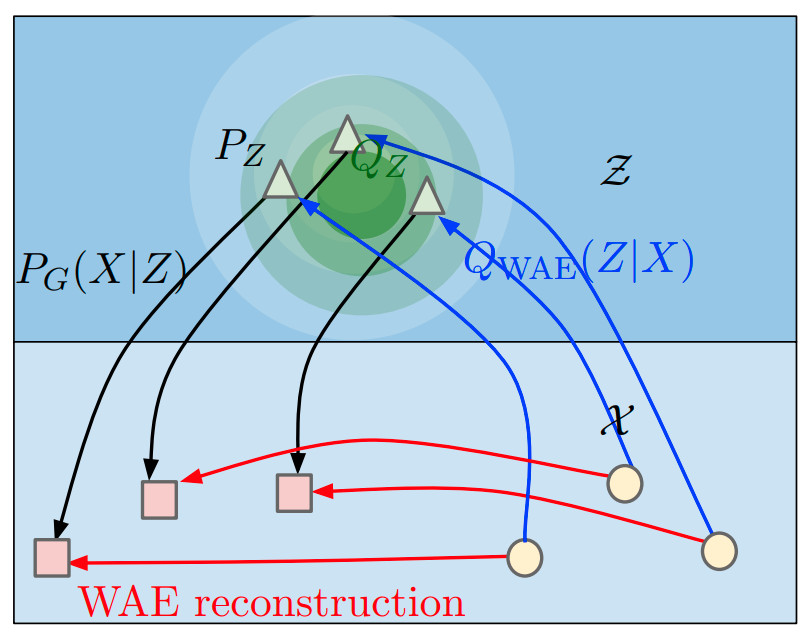
\includegraphics[width=0.50\textwidth,keepaspectratio]{./figures/wae_structure}
\end{center}
\begin{itemize}
  \item Loss function:
\end{itemize}
\begin{align*}
  D_{WAE}(P_X, P_G) := \inf_{Q(Z|X)\in\mathcal{Q}} \mathbb{E}_{P_X}\mathbb{E}_{Q(Z|X)}\left[c(X, G(Z))\right] + \lambda \cdot \mathcal{D}_Z(Q_Z, P_Z)
\end{align*}
\end{frame}
%-----------------------------------------------------------------------------
\begin{frame}
\frametitle{Different penalties, different WAEs (1/3)}
\begin{itemize}
  \item Setting $$ \mathcal{D}_Z(Q_Z,P_Z) = D_{JS}(Q_Z, P_Z) $$
%  \begin{center}
  \vspace*{-\baselineskip}
  \item[]$\rightarrow$ we obtain WAE-GAN
  \item[](WAE using a GAN\footnote{Generative Adversarial Network \cite{gan}}-based penalty)
%  \end{center}
  \bigskip
  \item where $D_{JS}(\cdot,\cdot)$ is the Jensen-Shannon Divergence:
  \begin{align}
    D_{JS}(Q_Z,P_Z) := \frac{1}{2} D_{KL}(Q_Z, \frac{Q_Z + P_Z}{2})
      + \frac{1}{2} D_{KL}(P_Z, \frac{Q_Z + P_Z}{2})
  \end{align}
  \item and $D_{KL}$ is the Kullback-Leibler Divergence:
  \begin{align}
    D_{KL}(Q_Z,P_Z) := \int Q_Z \log \left( \frac{Q_Z}{P_Z}\right )
  \end{align}
\end{itemize}
\end{frame}
%-----------------------------------------------------------------------------
\begin{frame}
\frametitle{Different penalties, different WAEs (2/3)}
\begin{itemize}
  \item Setting $$ \mathcal{D}_Z(Q_Z,P_Z) = MMD_k(Q_Z, P_Z) $$
  \vspace*{-\baselineskip}
  \item[]$\rightarrow$ we obtain WAE-MMD
  \item[] (WAE with Maximum Mean Discrepancy as penalty)
  \bigskip
  \item where $MMD_k(\cdot,\cdot)$ is the Maximum Mean Discrepancy with \textit{characteristic} kernel $k$:
  \begin{align*}
    MMD_k(Q_Z,P_Z) := \Big\| \int_{\mathcal{Z}} k(z, \cdot)dQ_Z(z) -
      \int_{\mathcal{Z}} k(z, \cdot)dP_Z(z)\Big\|_{\mathcal{H}_k}
  \end{align*}
\end{itemize}
\end{frame}
%-----------------------------------------------------------------------------
\begin{frame}
\frametitle{Different penalties, different WAEs (3/3)}
\begin{itemize}
  \item Setting $$ \mathcal{D}_Z(Q_Z,P_Z) = \underbrace{\left\| \mu_{P_Z} - \mu_{Q_Z} \right\|^2 +
    \Tr \left( \Sigma_{P_Z} + \Sigma_{Q_Z} -
    2(\Sigma_{P_Z}\Sigma_{Q_Z})^{\frac{1}{2}} \right)}_{\text{2-Wasserstein distance between two multivariate normal distributions \cite{frechet}}} $$
  \item[] $\rightarrow$ we obtain WWAE
  \item[] (WAE with 2-Wasserstein penalty)
  \bigskip
\end{itemize}
\end{frame}
%-----------------------------------------------------------------------------
\begin{frame}
\frametitle{Results on MNIST}
\begin{itemize}
  \item Example interpolations on MNIST with ACAI + WWAE:
\end{itemize}
\begin{center}
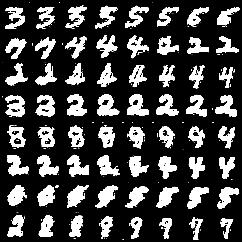
\includegraphics[width=0.5\textwidth,keepaspectratio]{./figures/01-mnist-interpolations}
\end{center}
\end{frame}
%-----------------------------------------------------------------------------
\begin{frame}
\frametitle{Conclusion}
\begin{itemize}
  \item
\end{itemize}
\end{frame}
%-----------------------------------------------------------------------------
\begin{frame}
\frametitle{Appendix - Wasserstein distance}

\end{frame}
%-----------------------------------------------------------------------------
%-----------------------------------------------------------------------------
%-----------------------------------------------------------------------------
%-----------------------------------------------------------------------------
%-----------------------------------------------------------------------------
\begingroup
\footnotesize
\begin{frame}
\frametitle{References}
\begin{thebibliography}{99}

\bibitem{pytorch}{Paszke, Adam, et al. "Automatic differentiation in pytorch." (2017).}
\bibitem{acai}{Berthelot, David, et al. "Understanding and improving interpolation in autoencoders via an adversarial regularizer." arXiv preprint arXiv:1807.07543 (2018).}
\bibitem{wae}{Tolstikhin, Ilya, et al. "Wasserstein auto-encoders." arXiv preprint arXiv:1711.01558 (2017).}
\bibitem{wwae}{Zhang, Shunkang, et al. "Wasserstein-Wasserstein auto-encoders." arXiv preprint arXiv:1902.09323 (2019).}
\bibitem{gan}{Goodfellow, Ian, et al. "Generative adversarial nets." Advances in neural information processing systems. 2014.}
\bibitem{frechet}{Dowson, D. C., and B. V. Landau. "The Fréchet distance between multivariate normal distributions." Journal of multivariate analysis 12.3 (1982): 450-455.}

\end{thebibliography}

\end{frame}
\endgroup
%-----------------------------------------------------------------------------

\end{document}
